\documentclass{article}
\usepackage[spanish]{babel}
\usepackage[utf8]{inputenc}
\usepackage{listings}
\usepackage[left=3cm,right=3cm,top=2cm,bottom=2cm]{geometry}
\usepackage{amsmath}
\usepackage[document]{ragged2e}
\usepackage{color}
\usepackage{graphicx}
\usepackage{float}

\begin{document}

\title{\Huge EC - Práctica 2}
\author{\Large Javier Gálvez Obispo}
\date{\large\today}
\maketitle

\section{Sesión de depuración Suma\_01\_S\_cdec}
  \begin{flushleft}
    {\large 4. ¿Qué modos de direccionamiento usa la instrucción \textbf{add (\%ebx,\%edx,4),\%eax}?
    ¿Cómo se llama cada componente del primer nodo? El último componente se llama escala.
    ¿Qué sucedería si lo eliminásemos?} \break

    Utiliza direccionamiento indexado y direccionamiento directo. \break
    offset(base, index, scale) \break
    M[offset + R[base] + R[index] * scale] \break
    El programa deja de funcionar correctamente.

    \vspace{\baselineskip}
    {\large 7. La instrucción \textbf{jne} en el programa original se podría cambiar por
    alguno de entre otros tres saltos condicionales (uno de ellos es sencillamente un
    mnemotécnico para el mismo código de operación) y el programa seguiría funcionando igual.
    ¿Cuáles son esos 3 mnemotécnicos? ¿Qué tendría que suceder para que se notaran diferencias
    en el original} \break

    Los otros 3 saltos que se pueden utilizar son: jnz, jg, ja. \break
    La variable resultado tendría otro valor al acabar el programa.
  \end{flushleft}


\section{Sesión de depuración Suma\_01\_S\_libC}
  \begin{flushleft}
    {\large 1. ¿Qué error se obtiene si no se añade \textbf{-lc} al comando de enlazar
    ¿Qué tipo de error es? (en tiempo de ensamblado, enlazado, ejecución...)} \break

    suma\_02\_S\_libC.o: En la función `\_start': \break
   /home/javi/DGIIM/EC/practica2/suma\_02\_S\_libC.s:26: referencia a `printf' sin definir \break
   /home/javi/DGIIM/EC/practica2/suma\_02\_S\_libC.s:30: referencia a `exit' sin definir \break

   Es un fallo de enlazado.

   \vspace{\baselineskip}
   {\large 2. ¿Qué error se obtiene si no se añade la especifación del enlazador dinámico al comando de enlazar?
   ¿Y si se indica como enlazador un fichero inexistente?
   ¿Qué tipo de error es? (en tiempo de ensamblado, enlazado, ejecución...)} \break

   \$: ld -m elf\_i386 suma\_02\_S\_libC.o -o suma\_02\_S\_libC -lc /lib/ld-linux.so.2 \break
   \$: ./suma\_02\_S\_libC \break
   bash: ./suma\_02\_S\_libC: No existe el archivo o el directorio \break

   Crea el ejecutable pero no deja ejecutarlo, es un fallo de ejecución. \break

   \$: ld -m elf\_i386 suma\_02\_S\_libC.o -o suma\_02\_S\_libC -lc -dynamic-linker /lib/ld-linux.so.3 \break
   \$: ./suma\_02\_S\_libC \break
   bash: ./suma\_02\_S\_libC: No existe el archivo o el directorio \break

   Crea el ejecutable pero no deja ejecutarlo, es un fallo de ejecución.
  \end{flushleft}

  \section{Popcount.c}
    \begin{flushleft}
      {\large 8. Gráfica comparación de optimizaciones de gcc para popcount.c}
    \end{flushleft}

  \begin{figure}[H]
    \centering
    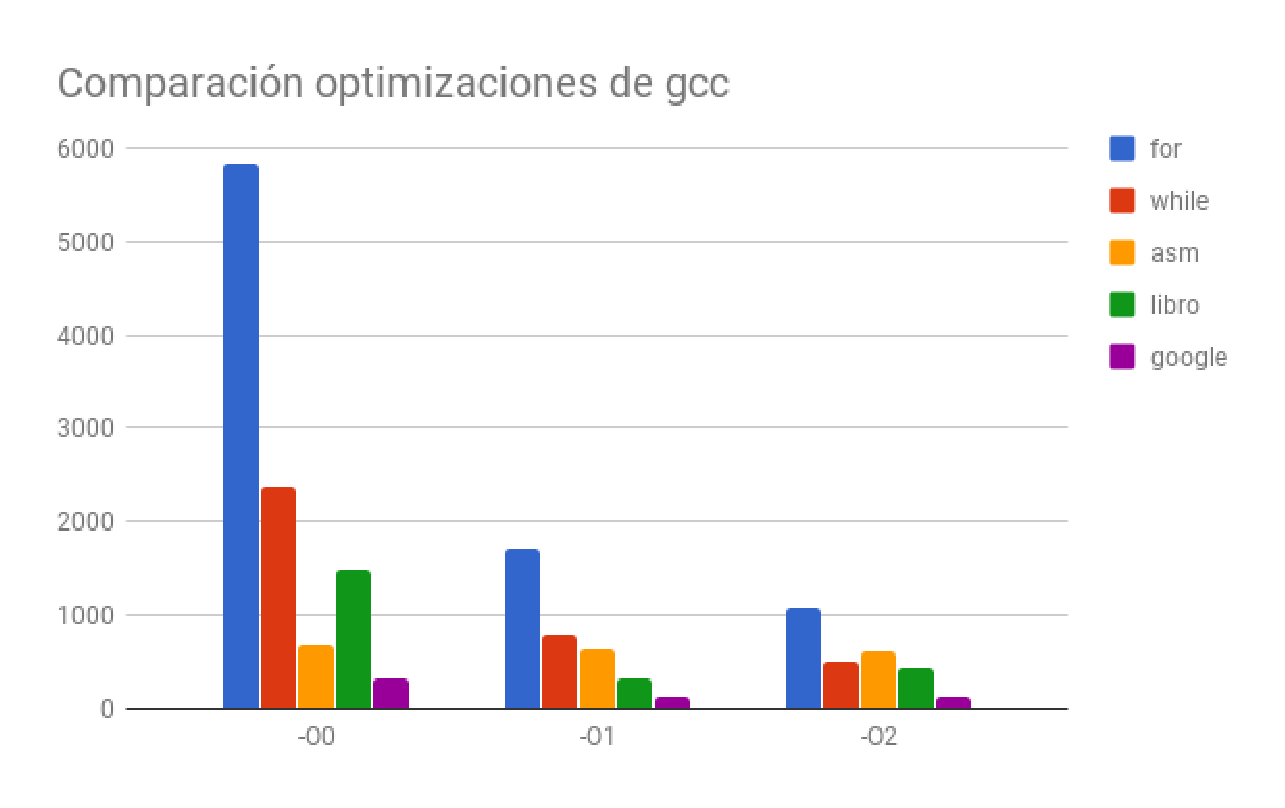
\includegraphics[width=\textwidth,height=\textheight,keepaspectratio]{popcount.eps}
    \caption{Gráfica rendimientos popcount.}
  \end{figure}


  \section{Parity.c}
    \begin{flushleft}
      {\large 1.Diseñar la fórmula sugerida en el cuarto párrafo de la sección 4.2.
      ¿Cómo se ha razonado ese cálculo?} \break

      El código se puede ver en el archivo parity.c. \break
      Siguiendo los consejos que nos dá el guión.  \break

      {\large 2. ¿Por qué necesitamos declarar la lista de enteros como \textbf{unsigned}
      ¿Qué problema habría si se declara como int? ¿Notaríamos en nuestro programa la diferencia?
      En caso negativo... ¿qué tendría que suceder para notar la diferencia?} \break

      Si se declara int en vez de unsigned el bit más significativo sería el del signo y nuestro programa
      dejaría de funcionar correctamente. \break

      {\large 3. En la 3ª versión (aplica máscara al final) se dejó pendiente comparar la 2ª para ver
      si la mejora es tan importante ¿lo es? ¿Para todos los niveles de optimización?} \break

      Como se puede ver en la gráfica (Figura 2) la tercera versión (libro, color amarillo) es más rápida,
      para todas las optimizaciones, que la segunda versión (while, color rojo). \break

      {\large 4. La 4ª versión (paso a ASM de la 3ª) probablemente sea la versión "extraña" de
      este ejemplo, porque no sea mejor que la anterior (incluso usando restricciones a registros)
      y/o porque tarde lo mismo independientemente del nivel de optimización. Intentar buscar
      explicación a ambas características, comparando los códigos ASM generados} \break


      Como podemos ver en la gráfica (Figura 2) la cuarta versión si que es más rápida que
      la tercera para -O0 y -O1 aunque para -O2 tardan lo mismo y si que tarda menos con las
      optimizaciones de gcc. \break

      {\large 8. En la 6º versión se usa un \textbf{clobber} EDX. Probar a quitarlo y recompilar
      con los tres niveles de optimización. ¿Pasa algo? ¿Para qué niveles? ¿Por qué? La explicación
      debe basarse en el código ASM generado.} \break

      Si lo quitamos para -O1 y -O2 deja de funcionar correctamente esa versión. \break
      Utiliza el registro \%ecx en vez de \%edx que el que nosotros utilizamos en nuestro código. \break

      {\large 9. Gráfica comparación de optimizaciones de gcc para parity.c}
    \end{flushleft}

    \begin{figure}[H]
      \centering
      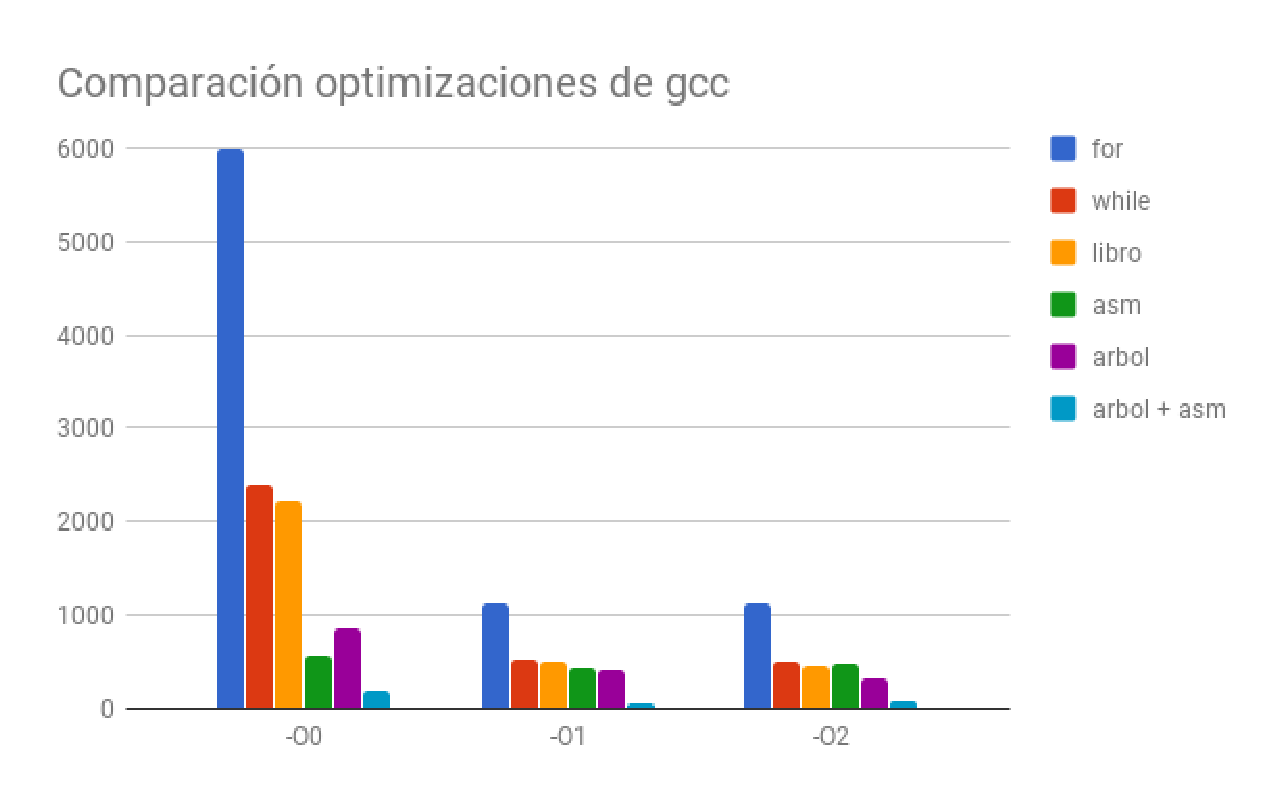
\includegraphics[width=\textwidth,height=\textheight,keepaspectratio]{parity.eps}
      \caption{Gráfica rendimientos parity.}
    \end{figure}
\end{document}
